\documentclass{article}



\usepackage[utf8]{inputenc}
\usepackage{graphicx}
\usepackage{blindtext}
%\usepackage{pgfgantt}
%\usepackage{pdflscape}
%\usepackage{xcolor}
\usepackage[table]{xcolor}
\rowcolors{3}{lightgray}{white}
%\usepackage{gensymb}
\usepackage{float}
\usepackage{etaremune}
\usepackage[acronym]{glossaries}
\usepackage[a4paper, portrait, margin=20mm]{geometry}
\usepackage[hidelinks]{hyperref}
\usepackage{enumitem}


\newacronym{io}{I/O}{Inputs and Outputs}
\newacronym{ice}{ICE}{Instrumentation and Control Engineering}
\newacronym{icse}{ICSE}{Industrial Computer Systems Engineering}
\newacronym{smc}{SMC}{Sintered Metal Corporation (Japan)}
\newacronym{plc}{PLC}{Programmable Logic Controller}
\newacronym{cpu}{CPU}{Central Processing Unit}
\newacronym{nc}{NC}{Normally Closed}
\newacronym{no}{NO}{Normally Open}
\newacronym{estop}{E-STOP}{Emergency Stop Button}
\newacronym{dc}{DC}{Direct Current}
\newacronym{ac}{AC}{Alternating Current}
\newacronym{led}{LED}{Light Emitting Diode}
\newacronym{ld}{LD}{Ladder-Logic}
\newacronym{st}{ST}{Structured-Text}
\newacronym{rt}{RT}{Real Time}
\newacronym{hmi}{HMI}{Human Machine Interface}
\newacronym{pc}{PC}{Personal Computer}
\newacronym{it}{IT}{Information Technology}
\newacronym{ot}{OT}{Operation Technology}
\newacronym{dword}{DWORD}{Double Word}
\newacronym{int}{INT}{Integer}
\newacronym{dint}{DINT}{Double Integer}
\newacronym{real}{REAL}{Real or Floating Point Number}
\newacronym{lsb}{LSB}{Least Significant Bit}
\newacronym{msb}{MSB}{Most Significant Bit}
\newacronym{i2c}{I$^2$C}{Inter-Integrated Circuit}
\newacronym{ip}{IP}{Internet Protocol}
\newacronym{ttl}{TTL}{Transistor-Transistor Logic}
\newacronym{dte}{DTE}{Data Terminal Equipment}
\newacronym{dce}{DCE}{Data Communication Equipment}
\newacronym{osi}{OSI}{Open Systems Interconnection}
\newacronym{bps}{Bps}{Bits per Second}
\newacronym{lan}{LAN}{Local Area Network}
\newacronym{lmu}{LMU2}{Lolly Machine Upgrade 2.0}
\newacronym{rgb}{RGB}{Red Green Blue}
\newacronym{ews}{EWS}{Engineering Work Station}
\newacronym{wap}{WAP}{Wireless Access Point}
\newacronym{fto}{FTO}{Fail to Open}
\newacronym{ftc}{FTC}{Fail to Close}
\newacronym{ll}{LL}{Ladder Logic}

% placeholder - makes a red X
\newcommand{\X}{
\textcolor{red}{X}
}

% note for graeme - makes a blue note for graeme
\newcommand{\GC}[1]{
\textcolor{blue}{NOTE FOR GRAEME - {#1}}
}

%note for henry - makes a purple note
\newcommand{\HD}[1]{
\textcolor{purple}{NOTE FOR HENRY - {#1}}
}

% cite reminder - makes a bold red CITE reminder
\newcommand{\remCite}{
\textcolor{red} {\textbf{CITE}} 
}


\makeglossaries

\usepackage[backend=biber,style=ieee,sorting=none]{biblatex}
\addbibresource{bibliography.bib}

\graphicspath{ {2_images/} }

% title page information
\title  {\begin{center}
            
\includegraphics[scale = 0.2]{murdochLogo} 
            \vspace{10mm}
            \\{\Huge The Lolly Machine Upgrade 2}
            \vspace{10mm}
            \\{\Huge Literature Review/ Background}
            \vspace{5mm}
            \\{\Large ENG470 - Engineering Honours Thesis}
            \vspace{40mm} 
            \\ Supervisor: Dr Graeme Cole
        \end{center}}
\author{Henry Davies}
\date{September 2022}

\begin{document}

% title page
\maketitle
\newpage

% table of contents page
\tableofcontents
\newpage

% list of figures page
\listoffigures
\newpage

% acronyms page
\printglossary[type=\acronymtype]
\newpage

\section{Introduction}
    The lolly machine is a demonstrating unit for the Murdoch University School of Engineering that sorts Allen's Kool Fruits\textsuperscript{TM} by colour. The intended purpose of the lolly machine is to showcase the capabilities of Industrial Computer Systems Engineering students. At this present time, the lolly machine is inoperable and in desperate need of an upgrade. 

The project plan contained in this document will outline the necessary actions required to upgrade the lolly machine to a state that is ready for demonstration while surpassing the functionality of the current design.

This document details the project plan of what has been affectionately named \textbf{The Lolly Machine Upgrade 2}, hereafter referred to as the LMU2.

    \newpage

\section{Mechanical}
    \subsection{Pneumatics}

    Most industrial operations require objects to be moved from one location to another - this is achieved through mechanical movement driven by prime movers \cite{parr2011hydraulics}. Prime movers are the power houses of industrial operations. Electric motors are a common choice for prime movers as rotary and linear movement can be achieved through either and or a direct or geared coupling to the motor shaft\cite{parr2011hydraulics}. Electric motors are not the only option as movement can be facilitated through subsequent flow of fluid - liquid and gas\cite{parr2011hydraulics}. Hydraulics is the name given to liquid-based systems and Pneumatics is the name given to air-based systems. The nature of the application will dictate whether an electric, hydraulic, pneumatic or a combination of each should be implemented. For example - pneumatics are common within the food processing industry as a leak in the pneumatic line will not spoil the food. Figure \ref{fig:pnemumaticSystem} illustrates a simplified overview of the necessary components required for a pneumatic system. 
    All mechanical movement within the lolly machine is driven by pneumatic actuators. As the lolly machine is portable, the pneumatic system supplying the machine will vary depending on location.
    
    \begin{figure}[H]
        \centering
        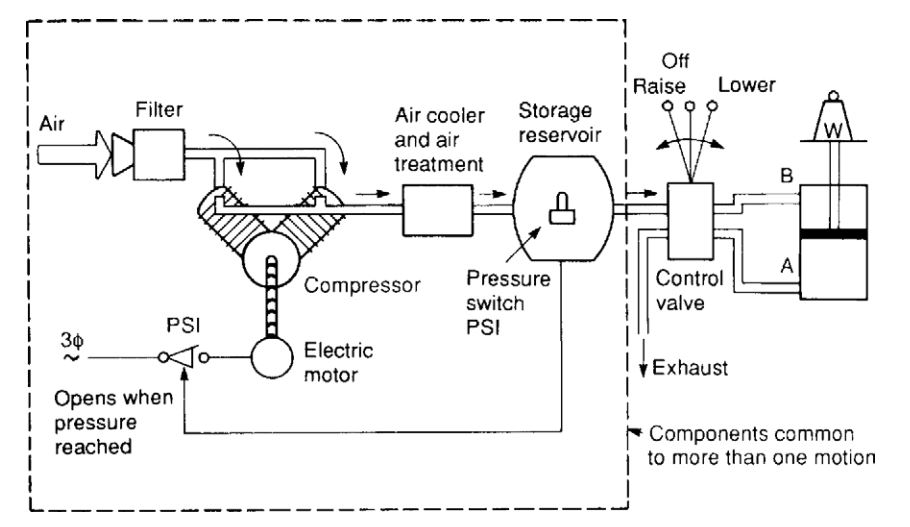
\includegraphics[scale = 0.6]{pneumaticSystem.JPG}
        \caption{A simplified overview of a pneumatic system~\cite{parr2011hydraulics}.}
        \label{fig:pnemumaticSystem}
    \end{figure}
    \newpage
    
\subsection{Linear Actuators}
    Linear actuators, as the name suggests, provides linear movement to push and/or pull objects within a given process. The linear actuators on the lolly machine are powered by pneumatics. The main components of a linear actuator are as follows:
    
    \begin{description} 
        \item\textbf{Rod:} connects the actuator to the outside environment.
        \item\textbf{Piston:} facilitates movement to the rod through applied pressure to either side.
        \item\textbf{Barrel:} houses the piston.
        \item\textbf{Extend Port:} when air enters, the rod will extend outwards.
        \item\textbf{Retract Port:} When air enters, the rod will retract inwards.
    \end{description}
    
    The fundamental concept is that the differential pressure between either side of the piston will cause it to move\cite{parr2011hydraulics}. The direction of movement is dependent on the flow of air through the extend and retract ports.
    
    \begin{figure}[H] 
        \centering
        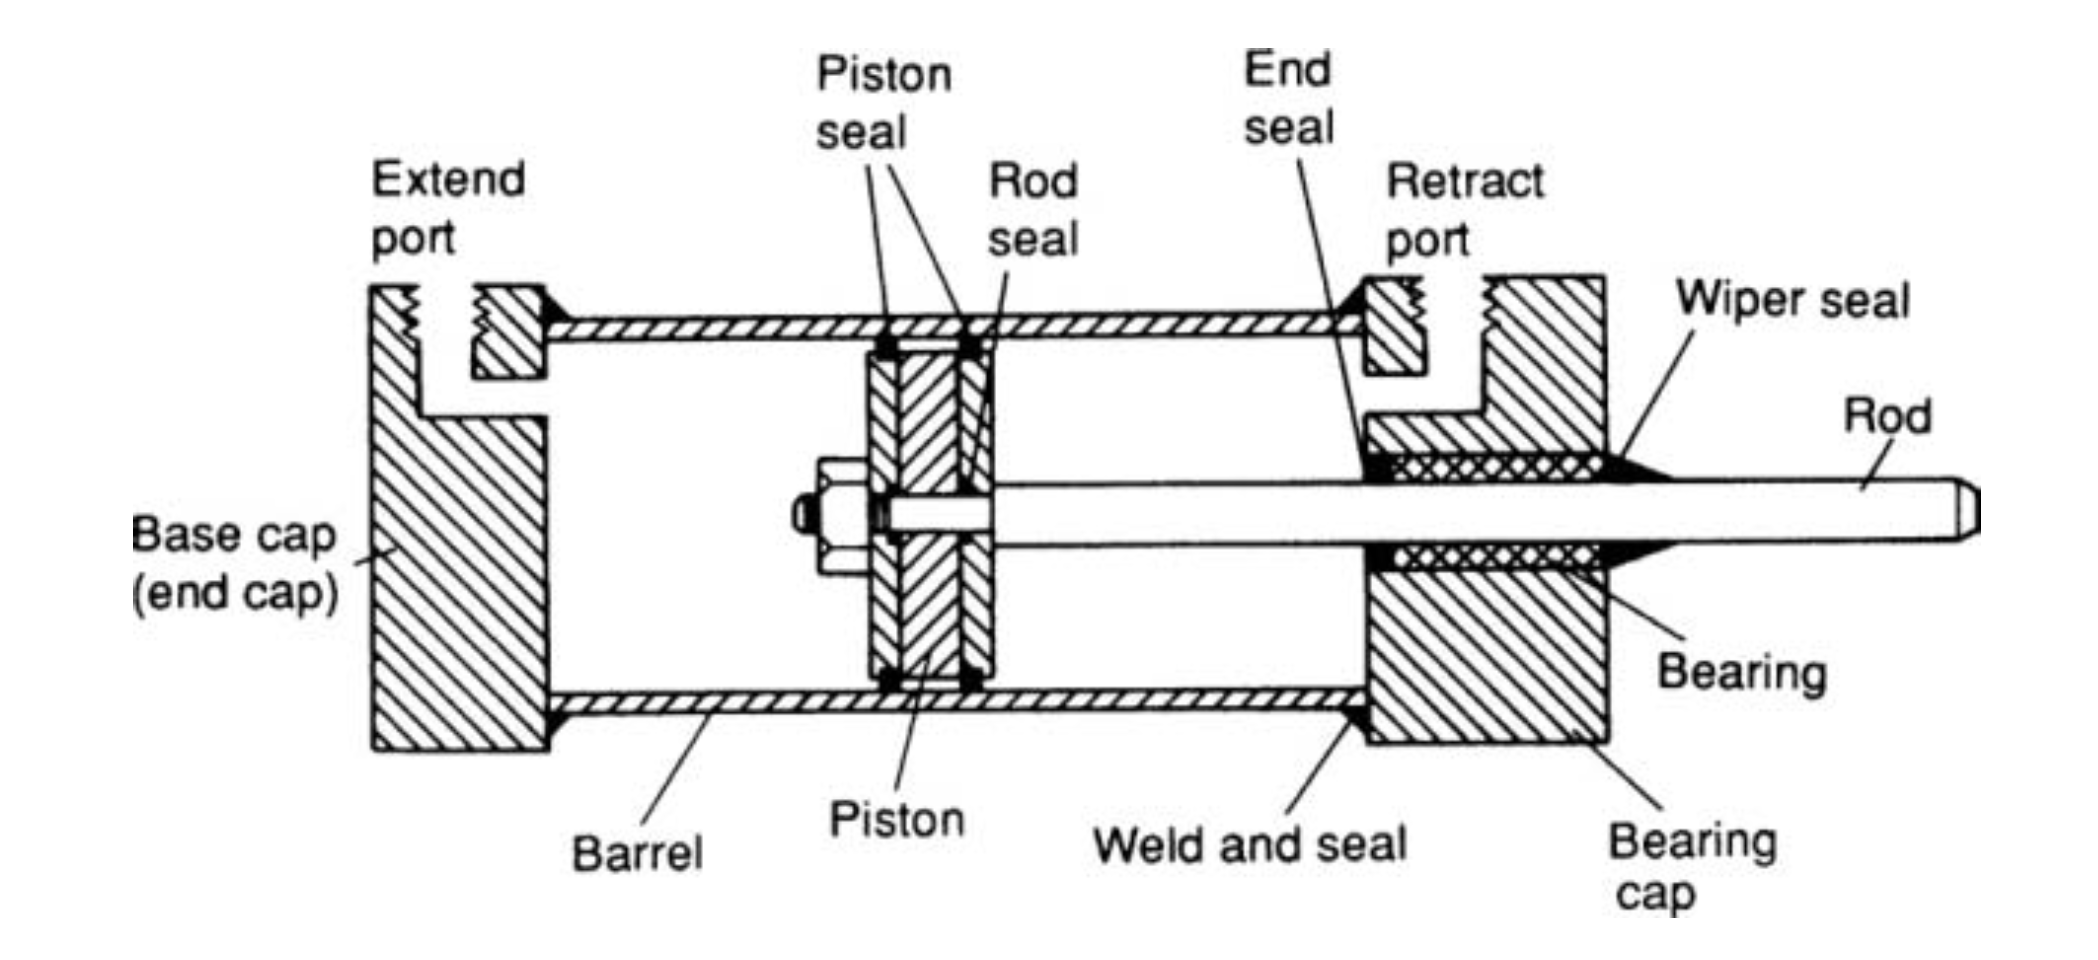
\includegraphics[width = 0.5\textwidth]{2_images/linearActuator.png}
        \caption{A cross section view of a linear actuator~\cite{parr2011hydraulics}.}
        \label{fig:linearActuator}
    \end{figure}
    
    There are eight linear actuators installed on the lolly machine. Three are used within the sorting process while five are required for dispensing. Figure \ref{fig:rejectAct} shows the linear actuator responsible for dropping lollies into the colour sensing shoot.

    \begin{figure}[H] 
        \centering
        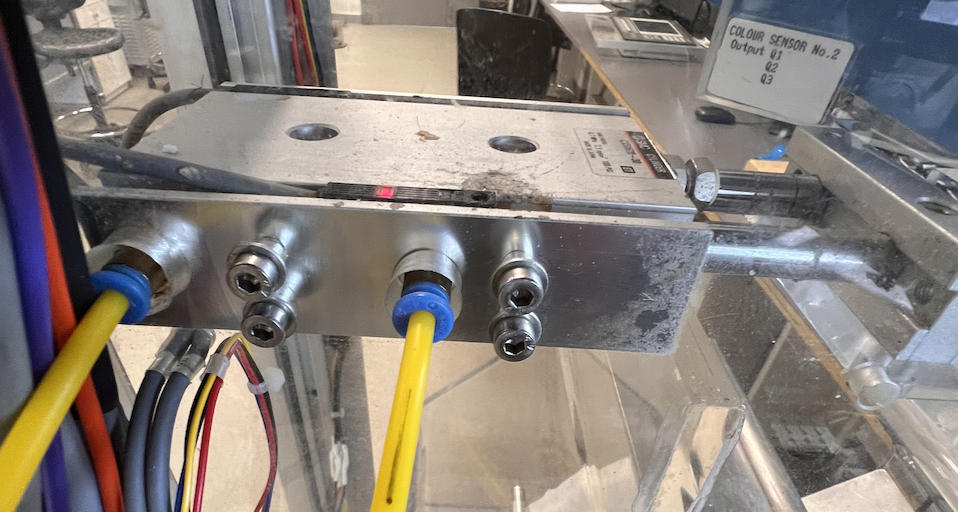
\includegraphics[width = 0.5\textwidth]{2_images/rejectAct.png}
        \caption{Lolly machine reject actuator.}
        \label{fig:rejectAct}
    \end{figure}        
\newpage     
\subsection{Rotary Actuators}
    Rotary actuators provide rotational movement to objects through a central shaft\cite{parr2011hydraulics}. Rotation can be restricted or unrestricted. A rack and pinion or vanes facilitate the turning action within the actuator\cite{parr2011hydraulics}. Rotary actuators within the lolly machine are driven by a single vane and restricted to 90$^{\circ}$\cite{smcRot}. Figure \ref{fig:rotaryActuator} shows a cross section of the \acrshort{smc} rotary actuators installed on the lolly machine. There are three rotary actuators installed on the lolly machine.
    
    \begin{figure}[H] % pushed to end
        \centering
        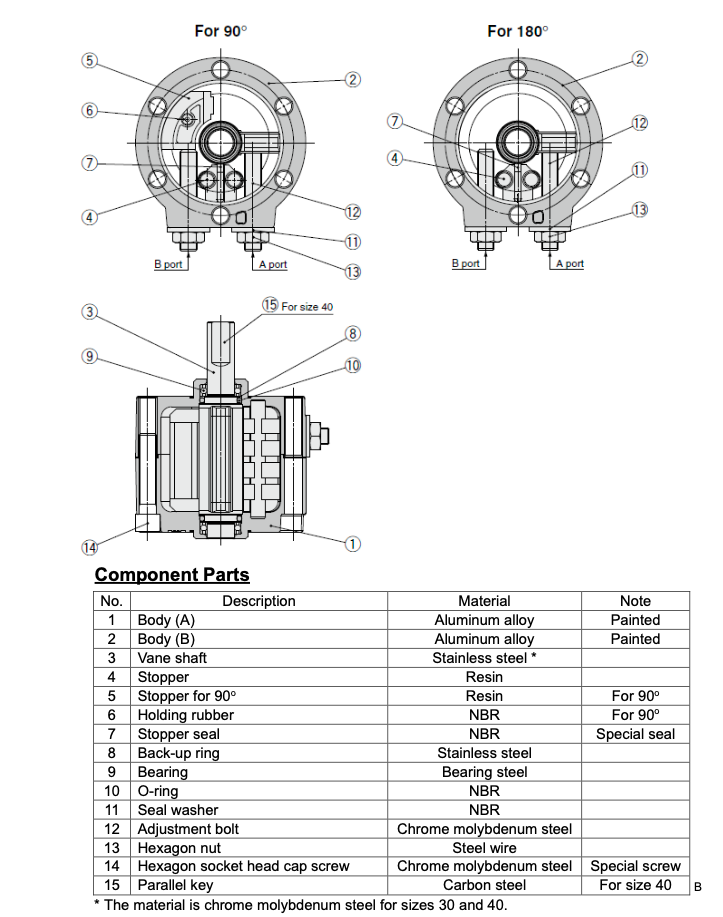
\includegraphics[scale = 0.4]{2_images/rotaryActuator.png}
        \caption{A cross section view of an \acrshort{smc} rotary actuator~\cite{smcRot}.}
        \label{fig:rotaryActuator}
    \end{figure}
\newpage
\subsection{Pneumatic Control Valves}
    Pneumatic control valves manage the air flow to pneumatic system peripherals. Control valves are defined by the number of ports, positions, and their control action\cite{parr2011hydraulics}. Figure \ref{fig:controlValves} compares two different types of valves - (a) shows a four-port two-position valve (4/2) while (b) shows a four-port, 3-position valve(4/2). Figure \ref{fig:controlValveConfig} shows a possible internal configuration for the 4/3 valve. It is important to note that the above mentioned figures do not represent typical pneumatic valve symbols and are included to illustrate the differences between various types of control valve configurations.
    
    \begin{figure}[H]
    \centering
    \begin{minipage}{0.45\textwidth}
        \centering
        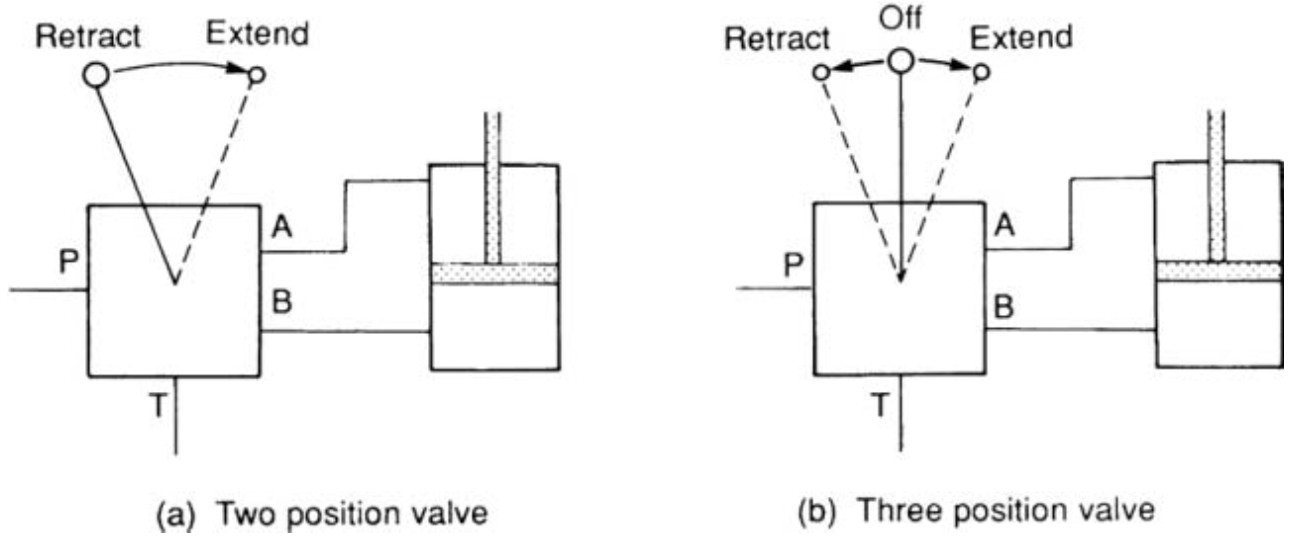
\includegraphics[width = 1\textwidth]{2_images/controlValves.png}
        \caption{Comparison between control valves~\cite{parr2011hydraulics}.}
        \label{fig:controlValves}
    \end{minipage}\hfill
    \begin{minipage}{0.5\textwidth}
        \centering
        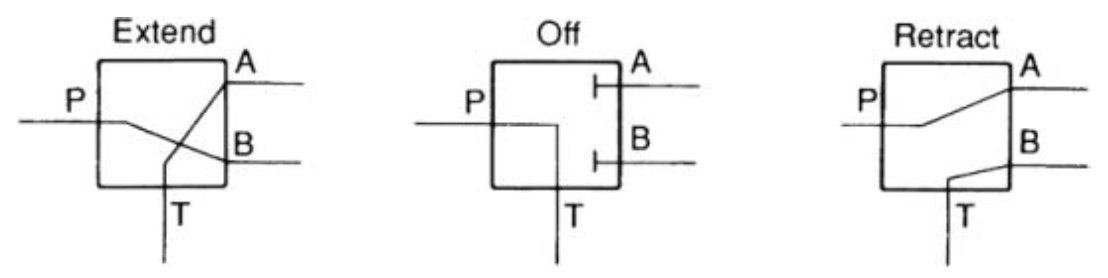
\includegraphics[width = 1\textwidth]{2_images/controlValveConfig.png}
        \caption{4/3 control valve switching configuration~\cite{parr2011hydraulics}.}
        \label{fig:controlValveConfig}
    \end{minipage}\hfill            
    \end{figure}      
    

    All actuators on the lolly machine are driven by 5/2 control valves, this means that each valve has two positions and 5 ports. Figure \ref{fig:5_2Valve} shows a 5/2 pneumatic valve symbol. Valve positions are shown by two square boxes (coloured red and green to clearly illustrate the different positions) each containing two arrows and a T. The arrows show the air flow direction between ports while the T represents a plug. The zigzag on the right hand side of the symbol illustrates a spring, indicating the the control valve is spring return. The rectangle with the diagonal line through the middle shows that a solenoid drives the control action. Figure \ref{fig:cylinderAB} shows the two possible positions of the cylinder.

    \begin{figure}[H]
    \centering
    \begin{minipage}{0.45\textwidth}
        \centering
        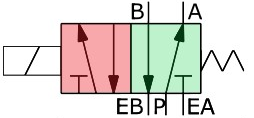
\includegraphics[scale = 0.5]{2_images/5_2Valve.png}
        \caption{A 5/2 pneumatic control valve \cite{5_2Valves}.}
        \label{fig:5_2Valve}
    \end{minipage}\hfill
    \begin{minipage}{0.5\textwidth}
        \centering
        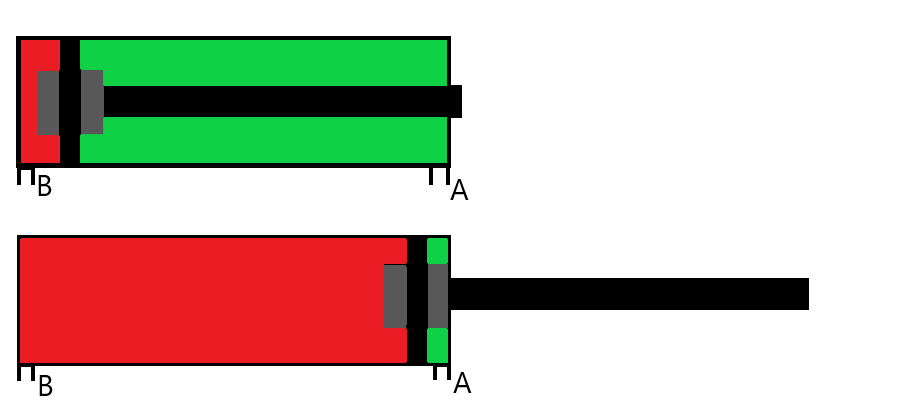
\includegraphics[width = 0.8\textwidth]{2_images/cylinderAB.png}
        \caption{Different cylinder positions. \\Position 1(Top) = Retracted. \\Position 2(Bottom) = Extended}
        \label{fig:cylinderAB}
    \end{minipage}\hfill            
    \end{figure}          
   
   The below position descriptions are in reference to Figure \ref{fig:5_2Valve}.
    \begin{description}
        \item\textbf{Position 1 - Green:}
        While the valve is in position 1 the pressure (P) port is connected to the (A) port and (B) port is connected to the exhaust line (EB).
        \item\textbf{Position 2 - Red:}
        While the valve is in position 2 the pressure (P) port is connected to the (B) side and (A) port is connected the exhaust line (EA). 
    \end{description}
    
 \newpage  
    The control action is what triggers the valve and can vary depending on the application, typical control actions include\cite{parr2011hydraulics}:
    \begin{itemize}
        \item Push Button
        \item Spring
        \item Lever
        \item Roller Limit Switch
        \item Pressure Line
        \item Solenoid
    \end{itemize}
    
    All control valves on the lolly machine are are triggered via solenoid driven pilot valves.
    \newpage

\section{I/O Devices}
    \acrfull{io}, as the name suggests, are the inputs and outputs of a control system. Inputs are often referred to as sensors as they are devices that translate a real world signal into something that the \acrshort{cpu} can make sense of - this typically consists of some sort of electrical signal (Voltage or Current). Outputs, on the other hand, are often referred to as "final control elements" or "actuators". Output devices are how the control system is able to interact with the outside world.\\
There are four main types of \acrshort{io}:


\begin{description}
    \item\textbf{Digital Inputs} - Binary input signals (On or Off).
    \item\textbf{Digital Outputs} - Binary output signals (On of Off).
    \item\textbf{Analog Inputs} - Variable electrical (voltage or current) inputs signals.
    \item\textbf{Analog Outputs} - Variable electrical (voltage or current) output signals.
\end{description}
    
    
The lolly machine \acrshort{io} is comprised of digital inputs and outputs. This section will provide a brief overview to all different types of digital \acrshort{io} that can be found on the lolly machine


\subsection{Inputs}
    \subsubsection{Limit Switches}
        Magnetically activated limit switches manufactured by \acrshort{smc} provide actuator position feedback. There are two limit switches installed on each actuator, one that activates when the actuator is fully extended and the other when it is fully retracted. The limit switches are installed within a track on the actuator and held in place by a small grub screw - this can be seen in Figure \ref{fig:rejectAct}.
        The limit switches have an internal solid state circuit that is activated when the piston is adjacent. The piston is made from a magnetic ferrous material which is what allows the switch to activate. 
        Figure \ref{fig:autSwShm} shows the internal electrical schematic of the \acrshort{smc} limit switches.
        
        \begin{figure}[H]
            \centering
            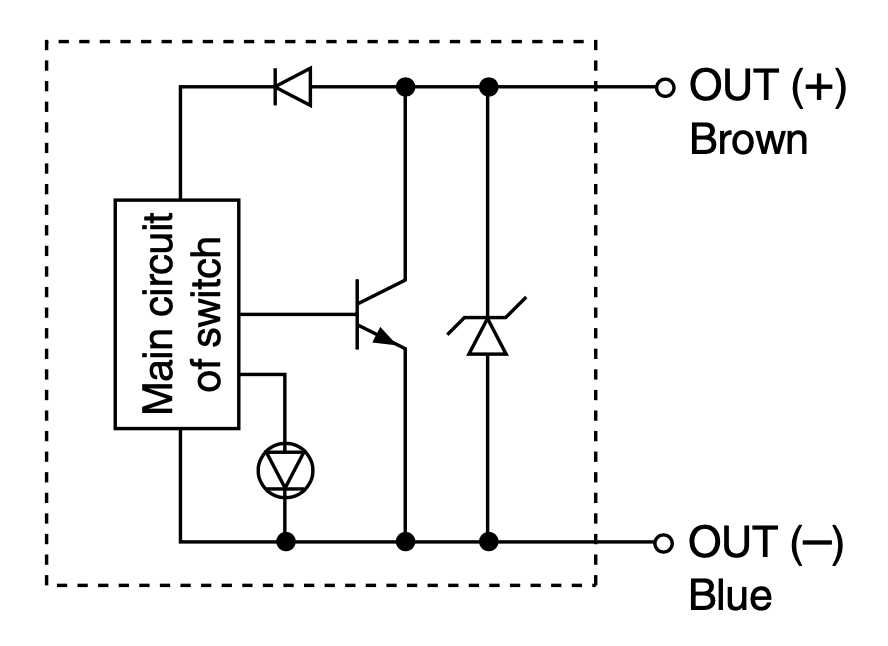
\includegraphics[scale = 0.4]{2_images/autSwShm.png}
            \caption{Internal electrical schematic of an \acrshort{smc} limit switch~\cite{smcRot}.}
            \label{fig:autSwShm}
        \end{figure}
    
        
        %PHOTO
    
    \subsubsection{Proximity Sensors}
        Two proximity sensors are installed on the lolly machine. The sensors determine whether or not a lolly is in situ. The proximity sensors installed on the lolly machine are capacitive; this allows the sensors to detect ferrous and non-ferrous materials. Figure \ref{fig:proxSens} illustrates the general function of a proximity sensors. In the case of the lolly machine, the proximity sensors are \acrshort{nc} which means that the output is on when the target is detected and off while the target is not.
    \begin{figure}[H]
    \begin{minipage}{0.35\textwidth}
        \centering
            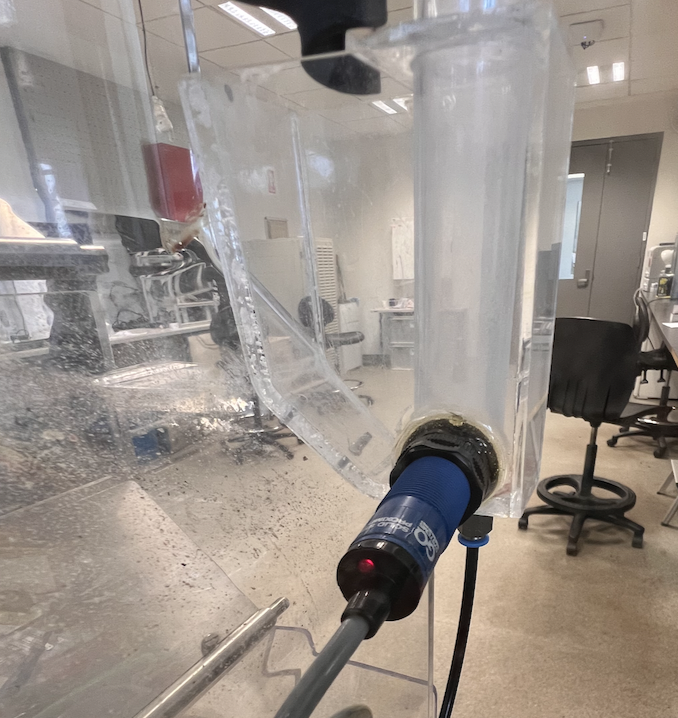
\includegraphics[scale = 0.4]{2_images/rejectProx.png}
            \caption{Lolly machine proximity sensor used to detect when a lolly is in the reject bucket.}
            \label{fig:rejectProx}
    \end{minipage}\hfill
    \begin{minipage}{0.35\textwidth}
        \centering
        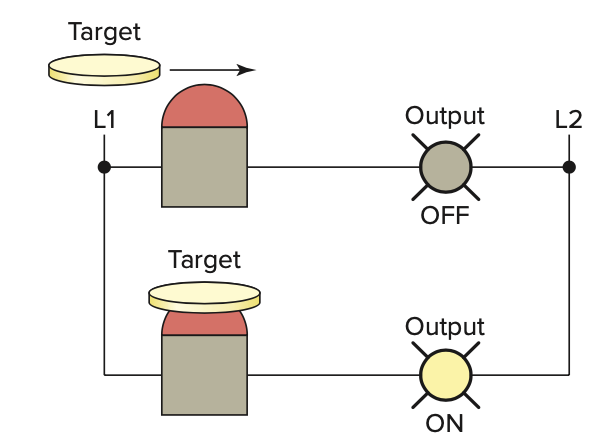
\includegraphics[width = 0.9\textwidth]{2_images/proxSens.png}
        \caption{Typical function of a proximity sensor \cite{petruzella2017programmable}.}
        \label{fig:proxSens}
    \end{minipage}\hfill 
    \end{figure}
 \newpage
    
    \subsubsection{Colour Sensors}
        Colour sensors determine colour through the hue, chrominance and luminance of an object \cite{sickCs}.
        Although the colour sensors used on the lolly machine can’t actually detect the complete range of colours which can be seen by us, the two colours sensors (3 digital signals from one sensor, and 1 digital signal from the second), are able to be “trained/calibrated” to provide an indication of a number of different colour matches.
        Figure \ref{fig:cs1} shows the electrical connections of one of the colour sensors while Figure \ref{fig:colSens} shows a picture of the colour sensors installed on the machine.

        \begin{figure}[H]
            \centering
            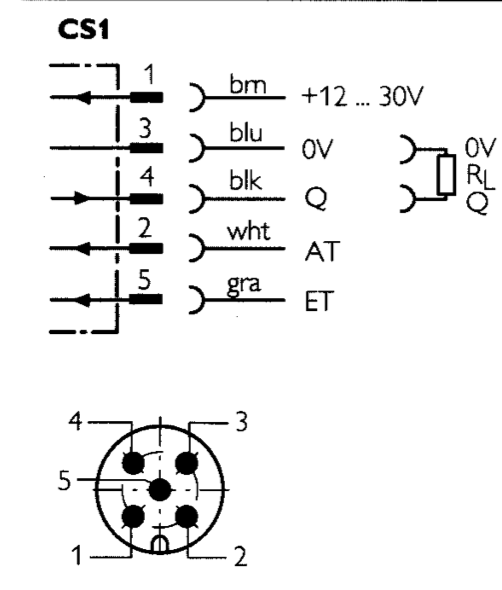
\includegraphics[scale = 0.4]{2_images/cs1.png}
            \caption{Electrical connections for a single output colour sensor \cite{sickCs}.}
            \label{fig:cs1}
        \end{figure}     
        
        \begin{figure}[H]
            \centering
            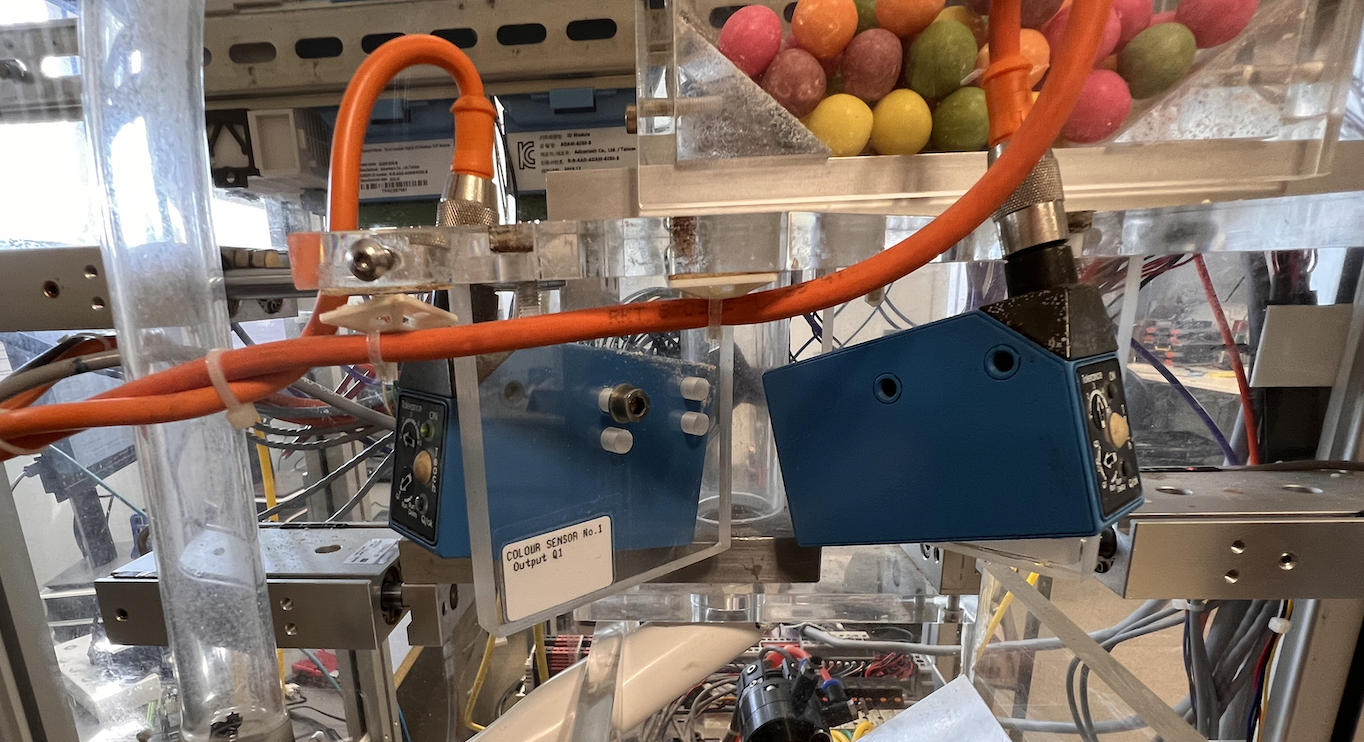
\includegraphics[scale = 0.4]{2_images/colSens.png}
            \caption{The two lolly machine colour sensors.}
            \label{fig:colSens}
        \end{figure}       

    
    \subsubsection{Buttons}
    Physical push buttons provide an interface between the operator and the machine where different buttons are linked to different machine functions. For example, an \acrfull{estop}, when pressed, will halt the operation of the machine and put it into error mode. While in error mode, the machine will cease to operate until it has been an given instruction by the user that it is safe to do so. The \acrshort{estop} is a \acrshort{nc} contact while the rest of the buttons on the machine are \acrshort{no}.
\newpage
    %Find a figure of a NO button - can probably find in the PLC book
    
\subsection{Outputs}
    \subsubsection{Solenoids - Pneumatic Valve}
    All pneumatic actuators on the lolly machine are activated by pneumatic control valves. The control valves are activated by an internal solenoid driven pilot valve.  The output device, from the perspective of the \acrshort{plc}, is the solenoid. The fundamental components of a solenoid are a wire coil and ferrous core. The ferrous core is located within the coil. When a \acrshort{dc} voltage is applied to the coil it behaves like a magnet, this is called an electromagnet. When the solenoid is switched, the ferrous core moves from one end of the solenoid housing to the other. The core is connected to the pilot valve which provides the necessary mechanical action to change the valve position, which in turn, moves the actuator. 
    
        \begin{figure}[H]
            \centering
            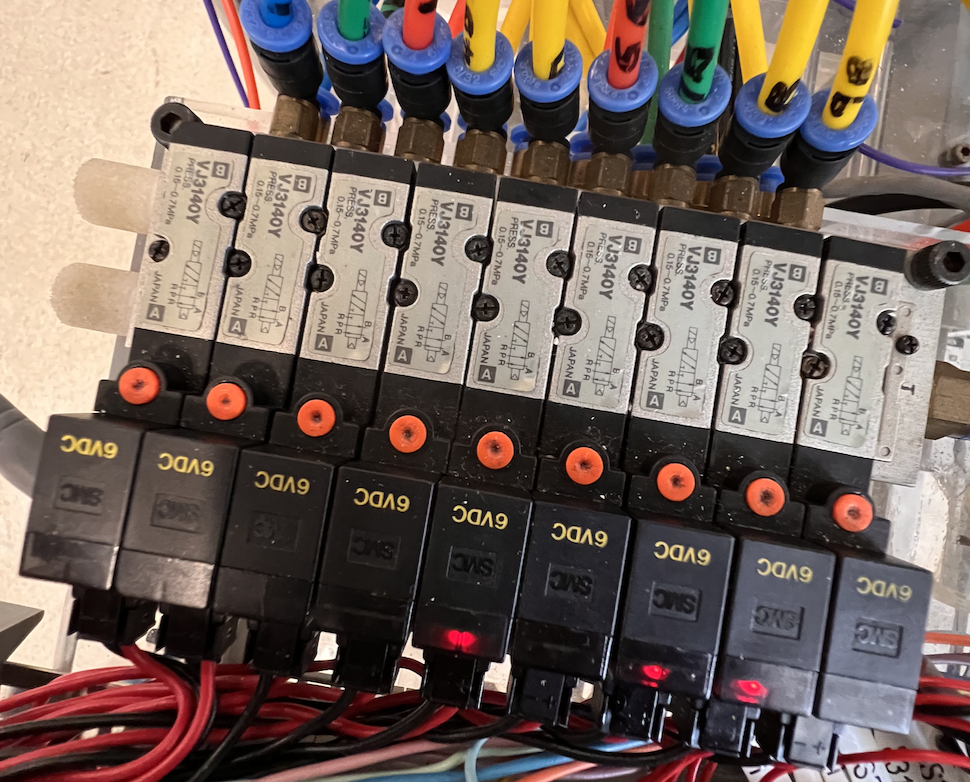
\includegraphics[scale = 0.5]{2_images/controlValvesPic.png}
            \caption{Solenoid pneumatic control valves mounted on manifold.}
            \label{fig:controlValvesPic}
        \end{figure} 
    \newpage
    \subsubsection{\acrshort{led} Indicators}
        A number of \acrshort{led} based lights are used on the lolly machine. The \acrshort{led}s are linked to specific machine states and will either be on, off  or flashing. \acrshort{led}s are robust, lasting much longer than previously used incandescent lights. As most \acrshort{led}s require only a couple of volts, all have internal series resistors which allows all \acrshort{led}s on the lolly machine to be directly controlled and switched by the \acrshort{plc}.
        
        
        \begin{figure}[H]
            \centering
            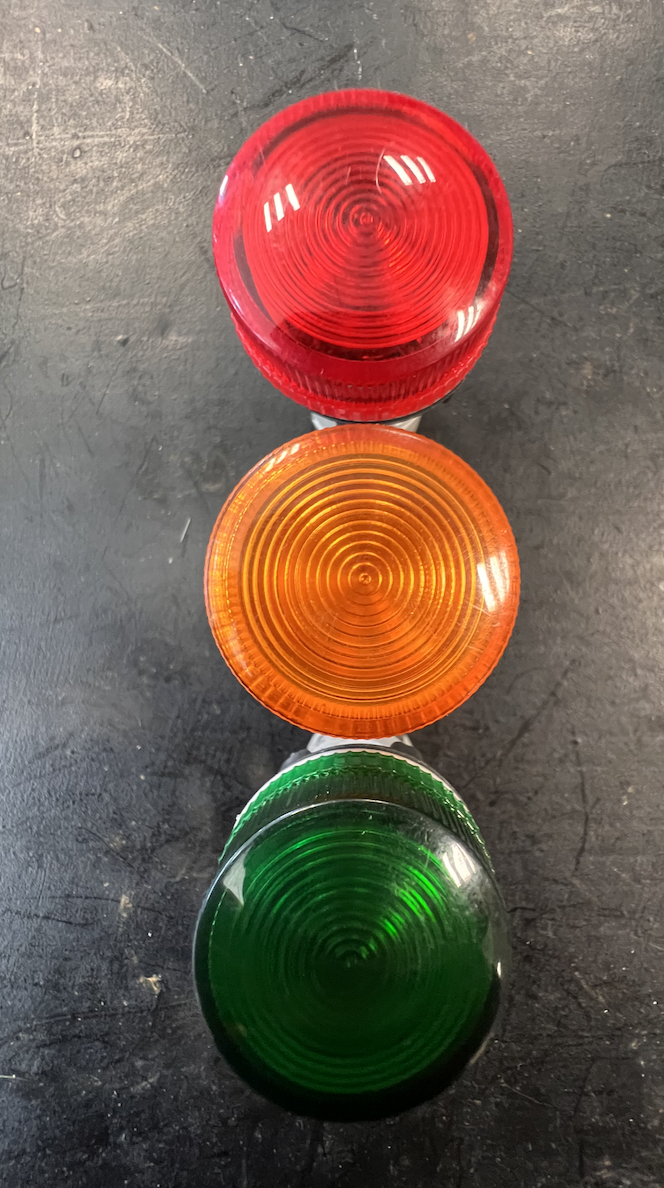
\includegraphics[scale = 0.3]{2_images/leds.png}
            \caption{Lolly machine \acrshort{led}s}
            \label{fig:leds}
        \end{figure} 
        

    \newpage
    
\section{Automatic Machines}
    %There are two main streams of process control - continuous and sequential\cite{dunn2006introduction}. Continuous control involves the constant monitoring and manipulation of dynamic systems while while sequential control is event based. Given the nature of the lolly machine, sequential control is the obvious choice for controlling the system \cite{dunn2006introduction}.

The lolly machine is, in essence, an automatic machine. This section investigates various components that facilitate the automation aspects of the project.

\subsection{Programmable Logic Controller}


    A \acrfull{plc} is an industrial controller/ computer that can be programmed to perform specific \acrshort{rt} tasks and can utilised for varying applications\cite{petruzella2017programmable}. A \acrshort{plc} performs these tasks through solving logic based operations\cite{petruzella2017programmable}.  E.g., if a water tank is filled to a level which is deemed "to high" turn off the water supply to the tank. A \acrshort{plc} interacts with the outside world through the use of either onboard or remote \acrshort{io}.
    
    Prior to the existence of \acrshort{plc}s, sequential based control was performed through relay\footnote{Relays are an electrical component comprised of a solenoid and contacts(\acrshort{no} and/or \acrshort{nc}), when the solenoid is energised the contacts change state.}-logic. Relay logic required multiple relays to be wired in a certain configuration allowing for the control of the system. Figure \ref{fig:relayLogic} shows an example of a relay-logic based control system\cite{petruzella2017programmable}. 
    \acrshort{plc}s provided a much cleaner, organised and easier to troubleshoot method of control as seen in Figure \ref{fig:plcLogic}.    
    
    \begin{figure}[H]
    \centering
    \begin{minipage}{0.35\textwidth}
        \centering
        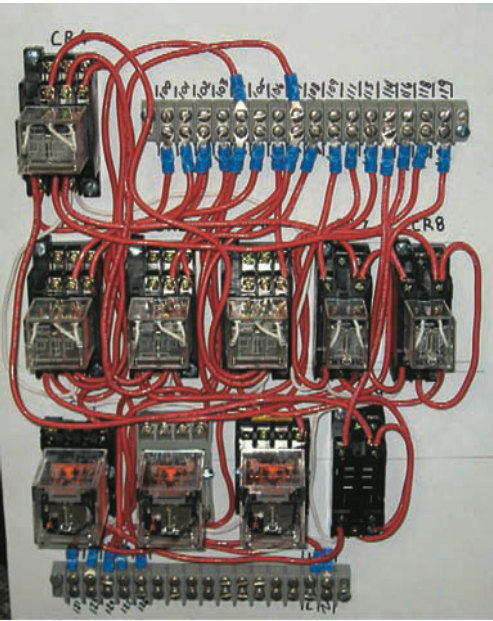
\includegraphics[width = 0.9\textwidth]{2_images/relayLogic.png}
        \caption{Relay logic based control system.~\cite{petruzella2017programmable}}
        \label{fig:relayLogic}
    \end{minipage}\hfill
    \begin{minipage}{0.35\textwidth}
        \centering
        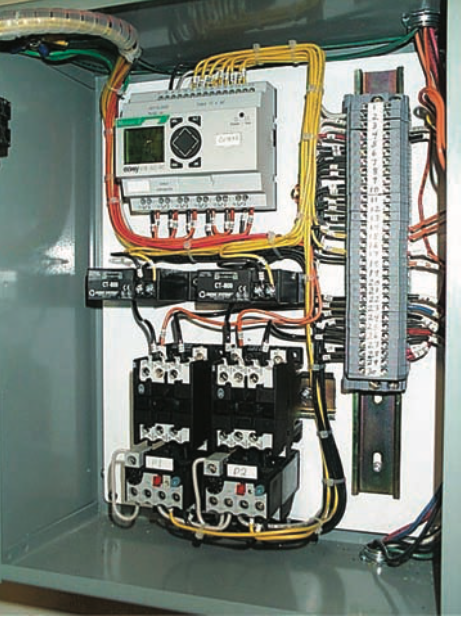
\includegraphics[width = 0.9\textwidth]{2_images/plcLogic.png}
        \caption{\acrshort{plc} based control system.~\cite{petruzella2017programmable}}
        \label{fig:plcLogic}
    \end{minipage}\hfill            
    \end{figure}   
    
    Originally, \acrshort{plc}s where exclusively programmed in a language called \acrfull{ld}\cite{petruzella2017programmable}. Ladder logic is a visual programming language based on electrical control schematics and was designed to be used by the same people who were building the relay logic based control systems ,electricians\cite{petruzella2017programmable}. In more recent times \acrshort{plc}s have become more sophisticated and can be programmed in a variety of languages including \acrfull{st} which is a text based language\cite{petruzella2017programmable}. 
    
    A \acrshort{plc}'s main components are a power supply, \acrlong{cpu}, and \acrshort{io} modules. \acrshort{io} modules can be located locally or remotely. Local \acrshort{io} is physically connected to the \acrshort{plc} while remote \acrshort{io} is connected to the \acrshort{plc} via a communication line, this is illustrated in Figure \ref{fig:localRemoteIo}.
    
    \begin{figure}[H]
        \centering
        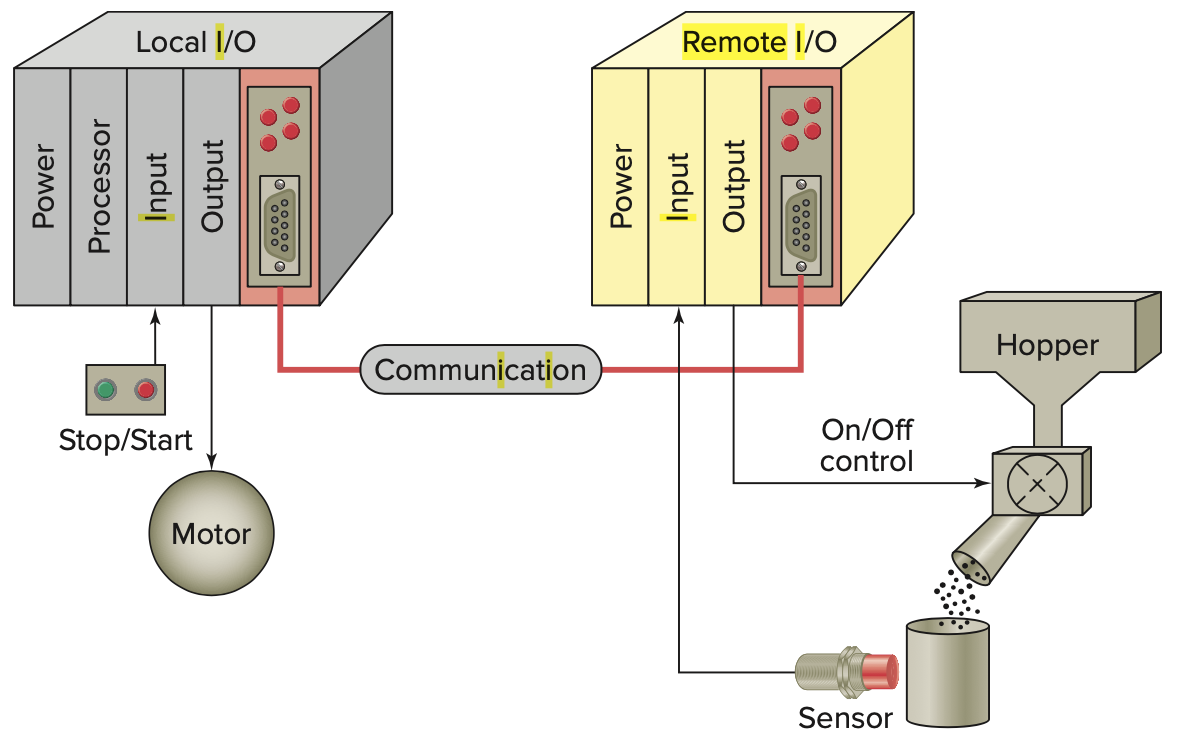
\includegraphics[width = 0.5\textwidth]{2_images/localRemoteIo.png}
        \caption{Local and remote \acrshort{io}}
        \label{fig:localRemoteIo}
    \end{figure}
  
    
\subsection{HMI}
    A \acrfull{hmi}, as the name suggests, is the interface between the machine and the operator. A \acrshort{hmi} is a screen that shows the machine state through graphics. An operator enters commands through the touch screen or a keyboard and mouse. \acrshort{hmi}s are programmable and can be used to control and monitor almost any machine\cite{petruzella2017programmable}. Typically, there is one \acrshort{hmi} per machine/ operator. It is not uncommon to have multiple \acrshort{hmi}s within a single factory. Figure \ref{fig:typHmi} shows an example of what a \acrshort{hmi} screen for a basic motor controller might look like.

    \begin{figure}[H]
        \centering
        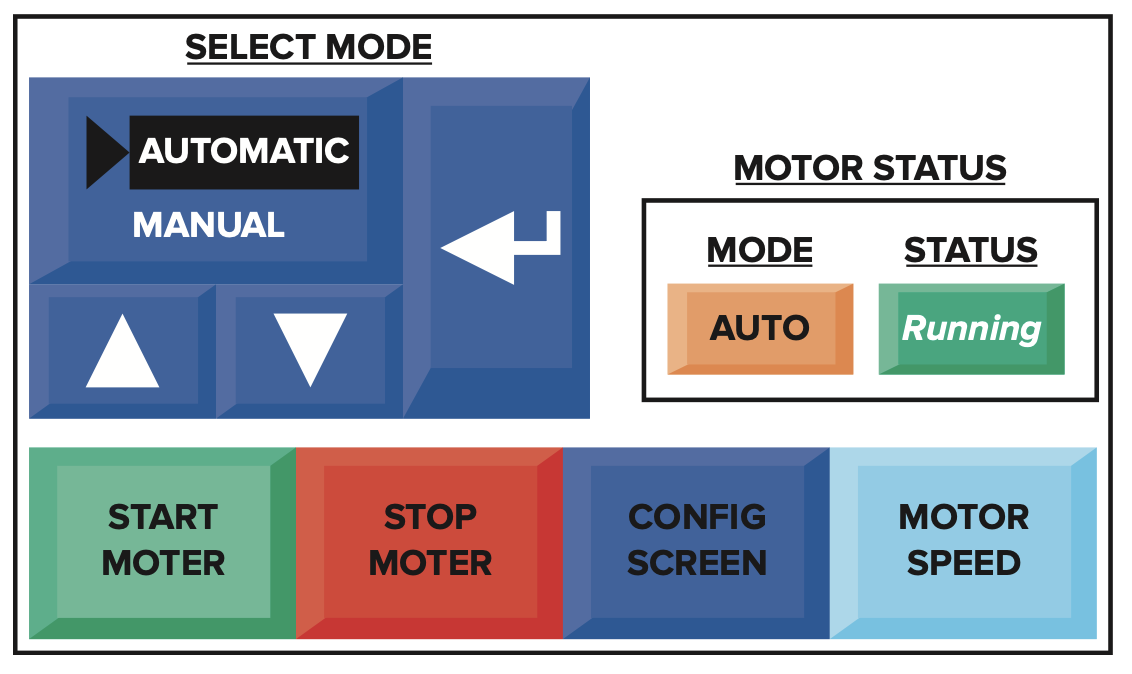
\includegraphics[width = 0.5\textwidth]{2_images/typicalHmi.png}
        \caption{A typical \acrshort{hmi} motor controller screen\cite{petruzella2017programmable}}
        \label{fig:typHmi}
    \end{figure}    
    
\subsection{Engineering Workstation}
    An engineering workstation is a \acrshort{pc} that has been set up for a engineer. The engineering workstation is connected to the \acrshort{ot} network and setup with all relevant software specific to the controlled process.  
\newpage    
\subsection{Microcontrollers}
    To understand what a microcontroller is, a few definitions must be made \cite{crisp2003introduction}.
    
\begin{description}
    \item{Integrated Circuits:} - An electronic circuit that is printed onto solid block. The circuit contains semi-conductor components. Integrated circuits are often referred to as chips.
    \item{Microprocessor:} - A microprocessor is part of a system, it is the central processing unit and is useless without surrounding circuitry and applied voltages.
    \item{Microprocessor-based System:} A microprocessor-based System is any system that is controlled by a microprocessor. 
\end{description}    
    
    A \textbf{microcontroller} is a complete microprocessor-based system built into an integrated circuit and is usually capable of controlling its own \acrshort{io} \cite{crisp2003introduction}.
    
    Microcontrollers are capable of performing an almost infinite list of tasks, e.g., controlling a wrist watch, monitoring and controlling a home irrigation system or controlling a robot. Some micorcontrollers, like the ones in a wrist watch or calculator,  can not be easily programmed after they leave the factory while other can.
    
    Similar to a \acrshort{plc}, micorcontrollers have onboard \acrshort{io} with the caveat being the hyper sensitivity to voltages above the standard operating voltage of the microcontroller which is typically 3.3 volts. Two micorcontrollers are used on the lolly machine - these are a Raspberry Pi and an Arduino.  
  
    \begin{figure}[H]
    \centering
    \begin{minipage}{0.4\textwidth}
        \centering
        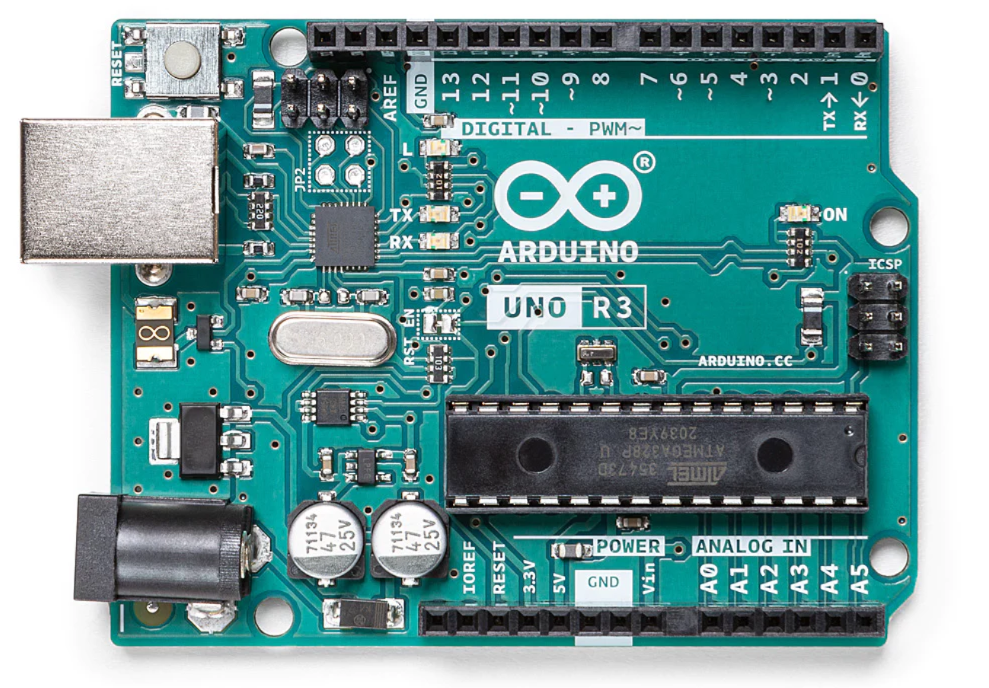
\includegraphics[width = 0.8\textwidth]{2_images/arduino.png}
        \caption{An Arduino~\cite{arduinoWeb}}
        \label{fig:arduino}
    \end{minipage}\hfill
    \begin{minipage}{0.4\textwidth}
        \centering
        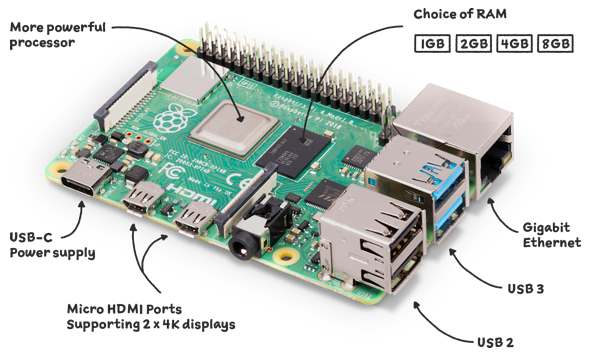
\includegraphics[width = 0.9\textwidth]{2_images/RaspPi.png}
        \caption{A Raspberry Pi~\cite{raspPiWeb}}
        \label{fig:raspPi}
    \end{minipage}\hfill            
    \end{figure}     

        

    

    \newpage  
    
\section{Communication}
    \subsection{Data Types}
    Data types represent different numerical formats within a process control system. The below list defines the basic data types used within a process control system.
    
    \subsubsection{BIT}
        Bits are binary values that can be either of two values, 1 or 0. Digital \acrshort{io} used within the lolly machine are all triggered by binary variables as the only two options are on (1) or off (0). 
    
    \subsubsection{BYTE}
        1 Byte is 8 bits. A BYTE can be represented in binary or by 2 hexadecimal characters.
    
    \subsubsection{WORD}
        1 Word is 2 Bytes which is 16 bits as illustrated in Figure \ref{fig:word}. A WORD can be represented in binary or by 4 hexadecimal characters.
        \begin{figure}[H]
            \centering
            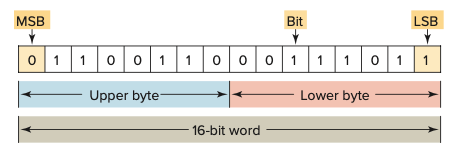
\includegraphics[width = 0.5\textwidth]{2_images/word.png}
            \caption{A 16 bit word \cite{petruzella2017programmable}.}
            \label{fig:word}
        \end{figure}           
        
    
    \subsubsection{\acrfull{dword}}
        1 Double Word is 2 Words which is 32 bits. A \acrshort{dword} can be represented in binary or by 8 hexadecimal characters.
 \newpage   
    \subsubsection{\acrfull{int}}
        An \acrshort{int} is a 16 bit number which can be either signed or unsigned. A signed \acrshort{int} ranges from -32,768 to 32,767 while an unsigned \acrshort{int} ranges from 0 to 65,535\cite{dataTypesSiemens}. Figure \ref{fig:int} illustrates how an 8 bit unsigned integer is represented in twos compliment - the same technique is applicable to 16 and 32 bit numbers.
        \begin{figure}[H]
            \centering
            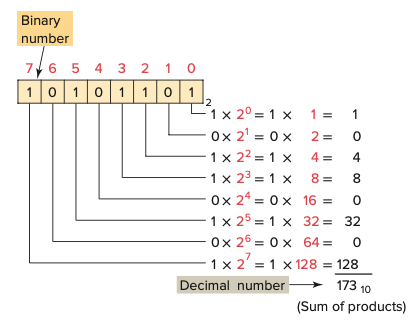
\includegraphics[width = 0.4\textwidth]{2_images/int.png}
            \caption{An 8 bit integer \cite{petruzella2017programmable}.}
            \label{fig:int}
        \end{figure}         
        
    
    \subsubsection{\acrfull{dint}}
        A \acrshort{dint} is a 32 bit number which can be either signed or unsigned. A signed \acrshort{dint} ranges from -2,147,483,648 to 2,147,483,647 while an unsigned is 0 to 4,294,967,295 \cite{dataTypesSiemens}. 
        
        \subsubsection{\acrfull{real}}
        A \acrshort{real} is a 32 bit number that represents real or floating point number. A \acrshort{real} can range from +/-1.18 x 10 $^{-38}$ to +/-3.40 x 10 $^{38}$ \cite{dataTypesSiemens}. A \acrshort{real} has three separate parts these are\cite{petruzella2017programmable}:
        
        \begin{description}
            \item\textbf{Sign}: 1 bit that defines the sign of the number.
            \item\textbf{Mantissa}: 23 bits, representing the significant figures.
            \item\textbf{Exponent}: 8 bits, representing the positive or negative power that the mantissa is raised.
        \end{description}
        
        \begin{figure}[H]
            \centering
            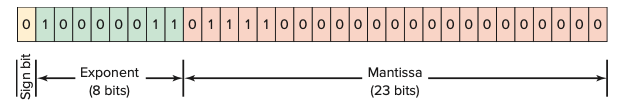
\includegraphics[width = 0.7\textwidth]{2_images/real.png}
            \caption{A \acrfull{real} word \cite{petruzella2017programmable}.}
            \label{fig:real}
        \end{figure}  
\newpage
\subsection{Serial Communication}
    Communication between devices can be achieved through serial communication. The base premise of serial communication is that data is sent one bit at a time \cite{frenzel2015handbook}. Bits are transmitted through a copper cable where differing voltage levels are inferred as either a 0 or 1\cite{frenzel2015handbook}. To understand serial communications properly there are a few terms that should be understood.
    \begin{description}
        \item\textbf{Baud Rate:} The number of bits that are transmitted or received per 1 second.
        \item\textbf{Telegram:} The complete set of data per transmission, comprising of 'n' number of bits which is dependent on the protocol.
        \item\textbf{\acrshort{lsb}:} The least significant bit in telegram.
        \item\textbf{\acrshort{msb}:} The most significant bit in telegram.
        \item\textbf{Parity Bit:} An optional check bit which is typically located at the \acrshort{lsb}. Parity can be either odd or even. Even parity means that there are an even number of 1s in a string while odd parity is an odd number of 1s in a string.
        \item\textbf{Start/ Stop-Bit:} A start bit defines the beginning of a telegram while a stop bit defines the end.
        \item\textbf{Half/ Full-Duplex} Half duplex means that data can be sent or received at any one point in time - data cannot be send and received synchronously. Full Duplex means that data can be sent and received at the same time.
    \end{description}
    Varying standards define different methods of serial communication. The lolly machine has two different serial communications standards. 
    
    % could also include spi and i2c but we will see. . . 
    \newpage
    \subsubsection{RS-232}
        RS-232 is a full-duplex, multi-wire, point-to-point system where a computer or terminal device, \acrfull{dte} communicates with various types of of \acrfull{dce}\cite{frenzel2015handbook}. 
        \begin{description}
            \item\textbf{Logic Levels:}
            \item0: +3V to +25V, Typically +5 to +12V
            \item1: -3V to -25V, Typically -5 to -12
        \end{description}
        
        An RS-232 port on the \acrshort{plc} provides a method of connection from the engineering workstation. The initial setup of the \acrshort{plc} must be made through this port as there are is no default \acrshort{ip} address.
        Figure \ref{fig:rs232Trans} illustrates an RS-232 data transmission.
        
        \begin{figure}[H]
            \centering
            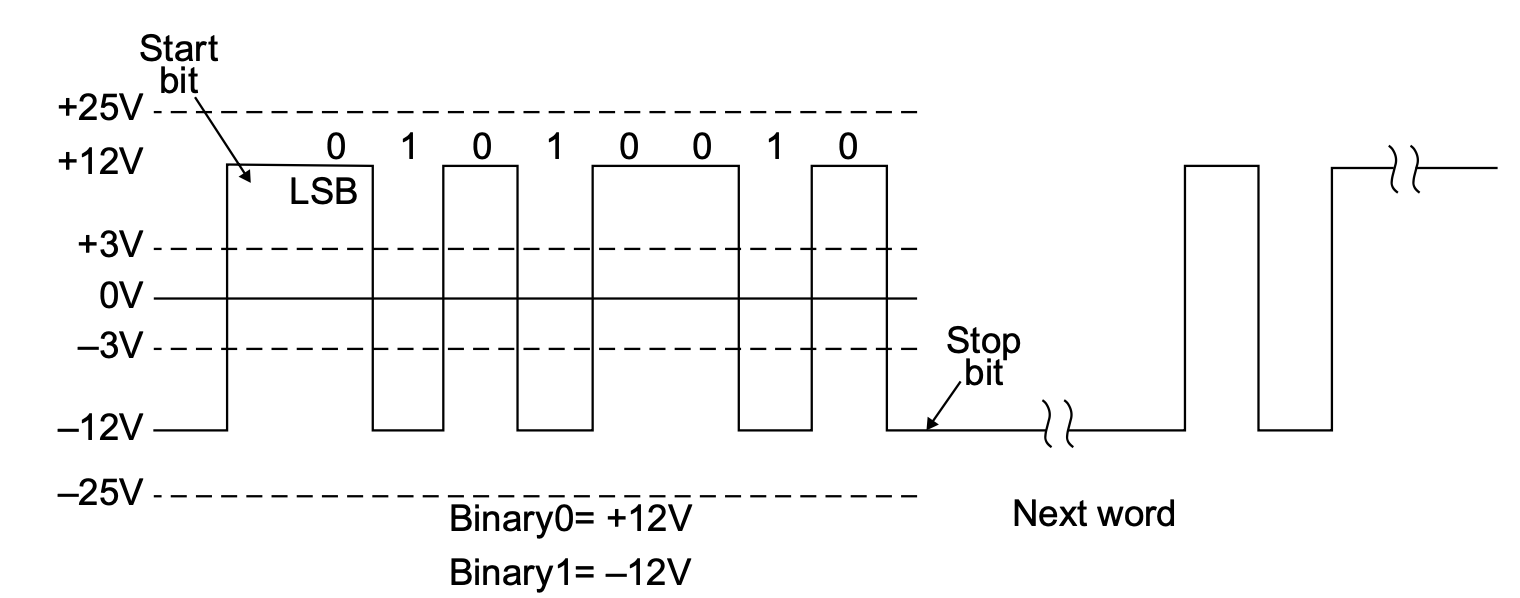
\includegraphics[width = 0.7\textwidth]{2_images/rs232Trans.png}
            \caption{A RS-232 data transmission~\cite{frenzel2015handbook}.}
            \label{fig:rs232Trans}
        \end{figure} 
    \newpage    
    \subsubsection{RS-485}
       RS-485 is a half-duplex, multi drop communication standard capable of supporting up to 32 nodes, each having transmitters and receivers. Voltages are taken across a differential pair which reduces the affect of noise on the system.  Data can be from 5 to 8 bits in length. Figure \ref{fig:rs485Nodes} shows a standard network configuration which includes two 120 ohm resistors which are used to combat reflections.

        \begin{figure}[H]
            \centering
            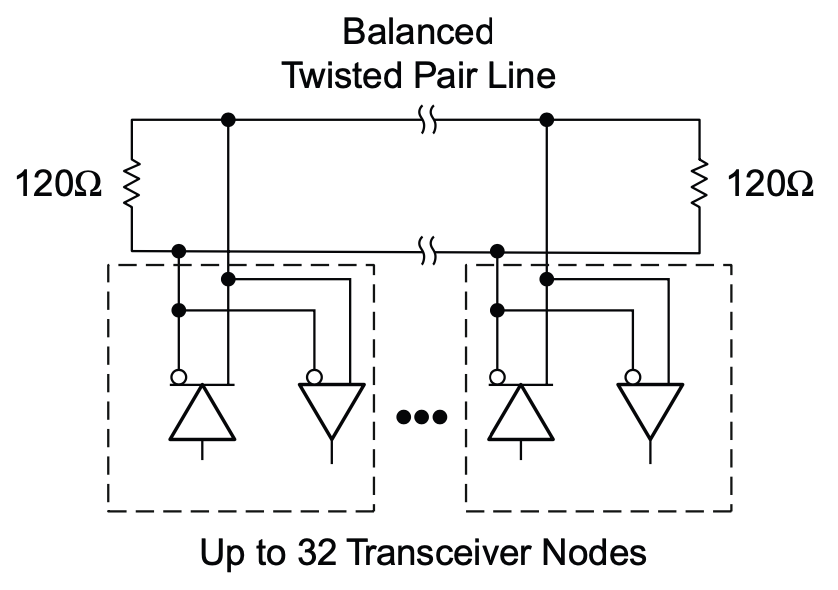
\includegraphics[width = 0.5\textwidth]{2_images/rs485Nodes.png}
            \caption{Configuration of a RS-485 network~\cite{frenzel2015handbook}.}
            \label{fig:rs485Nodes}
        \end{figure}        
       
       
        \begin{description}
            \item\textbf{Logic Levels:}
            \item0: +1.5V to +6V
            \item1: -1.5V to -6V
        \end{description}       
       
        An RS-485 port on the \acrshort{plc} is utilised to communicate with the Arduino through a RS-485 to \acrshort{ttl} converter.
     
\newpage    
\subsection{Ethernet}
    Ethernet, also known as IEEE 802.3, is a commonly used communication standard that governs the Physical and Data-Link Link layers (in relation to the \acrshort{osi}\footnote{The \acrshort{osi} model provides a framework that describes how applications can communicate over a wired \acrshort{lan}\cite{scott2021networking}.} model shown in Figure \ref{fig:osi}) of a wired \acrshort{lan}\cite{scott2021networking}. A wired \acrfull{lan} is a group of network devices that are connected on a local Ethernet network.  
    
        \begin{figure}[H]
            \centering
            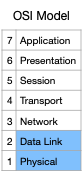
\includegraphics[width = 0.1\textwidth]{2_images/osi.png}
            \caption{The \acrshort{osi} model\cite{scott2021networking}.}
            \label{fig:osi}
        \end{figure} 
    
    An Ethernet network is established through physical cabling. Cabling can be coaxial, twisted copper pairs of fibre optic \cite{scott2021networking}.
    
    All devices on the lolly machine support Ethernet, subsequently all devices are on the same \acrshort{lan}.
    
    Each Ethernet device has a unique address which is called an \acrshort{ip} address. An \acrshort{ip} address is a four-octet, eight-bit address\cite{scott2021networking}.  
    
            \begin{figure}[H]
            \centering
            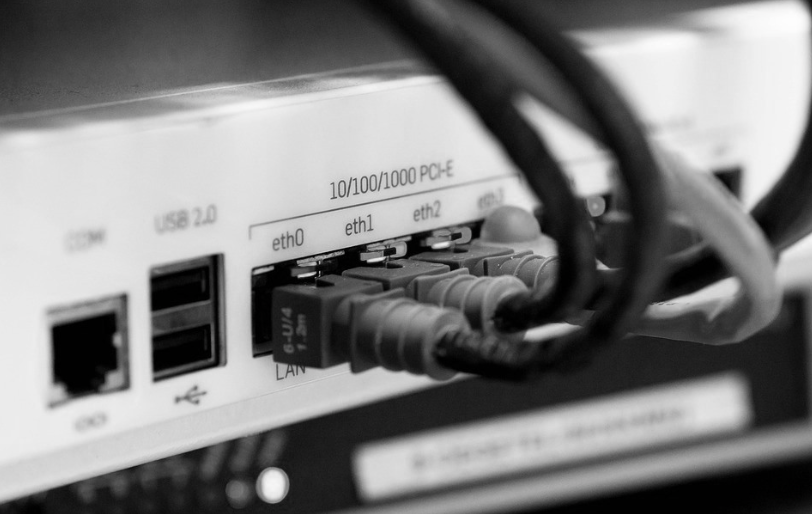
\includegraphics[width = 0.6\textwidth]{2_images/ethernetCables.png}
            \caption{Ethernet cables plugged into a network switch\cite{scott2021networking}.}
            \label{fig:ethenetCables}
        \end{figure} 
\newpage    
\subsection{Modbus}
    Modbus is an open-source \footnote{Open-source means that the developers have made the protocol available to the public. This allows third parties to use the protocol in their own products.} communication protocol that was produced by Modicon \cite{frenzel2015handbook}. Modbus was originally used exclusively in serial networks (RS-232 and RS-485) but has now expanded to TCP/IP which runs over an Ethernet network\cite{frenzel2015handbook}. 
    
    There are two main types of devices in a Modbus network, the Master and Slave\cite{frenzel2015handbook}. The Master can request data from a slave but not vice versa. A Master cannot request data from another master and a slave cannot request data another slave. Some devices like \acrshort{plc}s can be Mater/Slaves allowing inter \acrshort{plc} communication and tiered hierarchy of control. E.g., the \acrshort{hmi} on the lolly machine controls the \acrshort{plc} and the \acrshort{plc} controls the remote \acrshort{io}. Modbus on an Ethernet network operates on the same principles as those describe above however, the terminology is slightly different. A Master device is referred to as a Client while a Slave device is referred to as a Server. A way to remember this is that a server "serves" the client.
    
    In a Modbus network, data is communicated between devices in single bits or in WORDs (2 BYTES). 
    The Modbus protocol has four different address types, these are as follows:
    
    \begin{description}
        \item\textbf{Coil:} 1 bit - Read/ Write Access
        \item\textbf{Discrete Input:} 1 bit - Read Only Access
        \item\textbf{Input Register:} 16 bit WORD - Read Only Access
        \item\textbf{Holding Register:} 16 bit WORD - Read/ Write Access
    \end{description}
    
    When the Master/ Client device requests data from the Slave/ Server, it does so with a function code. The function code lets the Slave/ Server know how to respond to the request. The below list shows what each code corresponds to. 
    
    \begin{center}
        \begin{tabular}{ c c }
         \textbf{Code} & \textbf{Name}\\ 
            01 & Read Coil Status\\
            02 & Read Input Status\\
            03 & Read Holding Registers\\
            04 & Read Input Registers\\
            05 & Force Single Coil\\
            06 & Preset Single Register\\
            07 & Read Exception Status\\
            08 & Diagnostics\\
            09 & Program 484\\
            10 & Poll 484\\
            11 & Fetch Comm. Event Ctr\\
            12 & Fetch Comm. Event Log\\
            13 & Program Controller\\
            14 & Poll Controller\\
            15 & Force Multiple Coils\\
            16 & Preset Multiple Registers\\
            17 & Report Slave ID\\
            18 & Program 884/M84\\
            19 & Reset Comm. Link\\
            20 & Read General Reference\\
            21 & Write General Reference\\
        \end{tabular}\\
    \end{center}

The Modbus TCP/IP communication protocol is used extensively throughout various components of the lolly machine. Figure \ref{fig:overView} shows how the Modbus communication protocol facilitates the overall network architecture of the project.

        \begin{figure}[H]
            \centering
            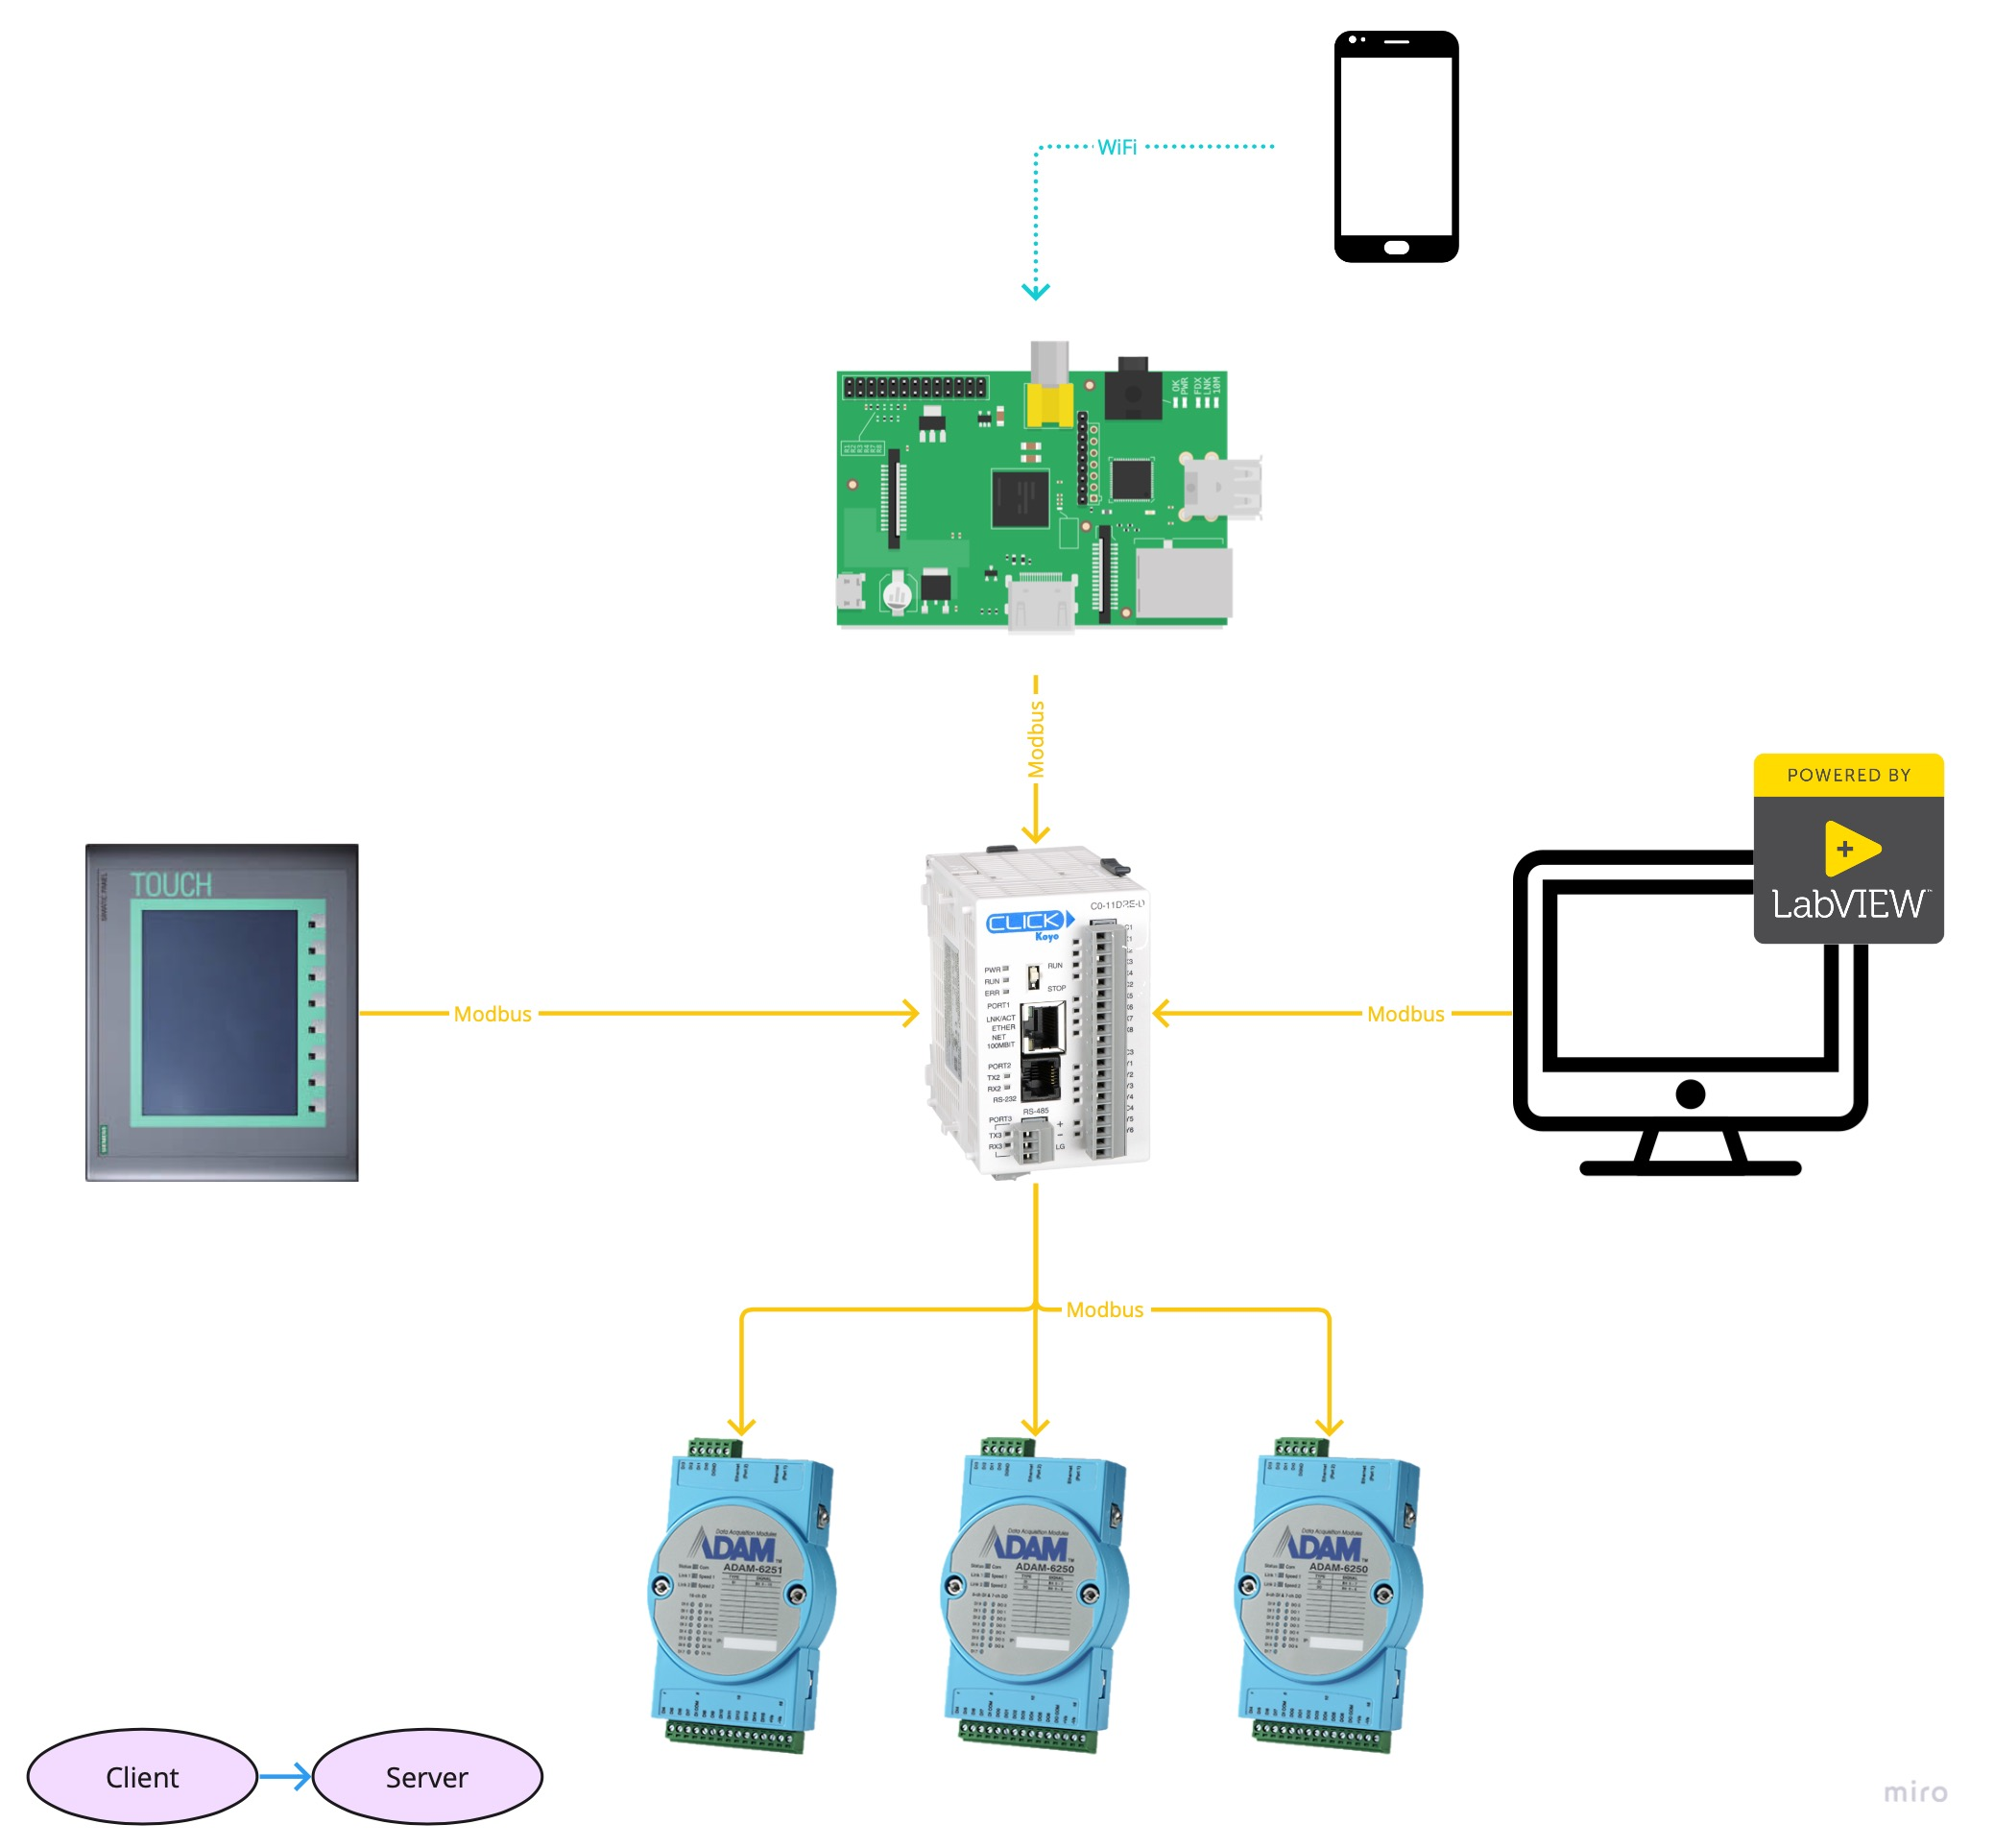
\includegraphics[width = 0.5\textwidth]{2_images/overView.jpg}
            \caption{Overview of the lolly machine network architecture.}
            \label{fig:overView}
        \end{figure} 
    \newpage
    
\section{Summary}
    Given the multifaceted nature of the \textbf{Lolly Machine Upgrade 2} there are many different terms, concepts and ideas that the reader must be aware of prior to understanding the main body of work to follow - the thesis report. This document has aimed to preface the reader with the required knowledge needed to be able to understand the proceeding thesis report. This way, the final body of work can focus on how and what was done rather than stopping ans starting all the time to explain ideas and concepts. Five main topics were discussed in this document. A basic introduction to pneumatics and the relevant devices were reviewed. Various types of \acrshort{io} devices onboard the machine were analysed. Specific components required for automatic machine operation were detailed and discussed and an introduction to relevant communication technologies was made. 
    \newpage
    
\addcontentsline{toc}{section}{References}
\printbibliography

\end{document}